\chapter{State of the Art}
\label{ch:stateart}
\section{Control Foundations}
\label{ch:navigation}

\subsection{Dynamical System and Control Input}
A control-affine dynamical system is written as
\begin{equation}
\dot x(t)=f(x(t))+g(x(t))u(t),
\label{eq:genericdynamics}
\end{equation}
where $x(t)\in\R^n$ is the state and $u(t)\in\mathcal U\subseteq\R^m$ is the control input. The function $f:\R^n\to\R^n$ describes the uncontrolled dynamics, while $g:\R^n\to\R^{n\times m}$ describes how the input changes the state. The set $\mathcal U$ represents actuator limits. A feedback controller chooses $u(t)$ from the available measurements to regulate the system or follow a reference~\cite{rootFeedback}.

This formulation applies to different robotic platforms. The state may contain position and velocity, while the input may represent a velocity command, force, or torque, depending on the control interface. Navigation additionally requires reaching a target or following a route while avoiding obstacles.

A state describes the quantities needed to predict how the system evolves. A measurement is the information available to the controller, which may be incomplete or noisy. Keeping these concepts separate is useful in robotics: a camera or range sensor does not directly reveal every velocity or disturbance acting on the platform. State estimation connects the sensor information to the variables required by the controller.

The input also depends on where the navigation algorithm sits in the control stack. A high-level velocity command can be passed to a lower-level controller that manages the actuators. Consequently, the same navigation objective may lead to different mathematical input definitions on different robots. The model and the safety condition must describe the interface that is actually controlled.

\subsection{Wind as an External Disturbance}
We are interested in navigation under wind, which perturbs the motion predicted by the nominal model. We represent its effect through an additive disturbance:
\begin{equation}
\dot x(t)=f(x(t))+g(x(t))u(t)+d(t),
\label{eq:disturbeddynamics}
\end{equation}
where $d(t)\in\R^n$ is the disturbance expressed in state-derivative coordinates. Components unaffected directly by wind can be zero. Thus $d(t)$ represents the effect of wind on the dynamics, rather than wind speed itself.

The disturbance is unknown and may vary over time. A controller designed for the nominal system can therefore develop tracking errors or lose obstacle clearance. This motivates a navigation policy that tolerates uncertainty and a safety mechanism that accounts for the disturbance.

Consider a vehicle attempting to hold a fixed position. A sustained wind can create a persistent mismatch between its command and observed motion, while a gust can cause a short transient deviation. Near an obstacle, both the size of that deviation and the time needed to correct it matter. A controller that eventually returns to the reference may still pass through an unsafe region during recovery.

This representation groups the disturbance by its effect on motion. It avoids requiring a detailed atmospheric model at this introductory stage, but it does not imply that wind has the same effect in every direction or at every speed. Later, disturbance-rejection methods use feedback, estimation, or learning to respond to this mismatch.

\subsection{PID and Model Predictive Control}
PID control adjusts the input using the tracking error $e(t)$:
\begin{equation}
u(t)=K_Pe(t)+K_I\int_0^t e(s)\,ds+K_D\dot e(t).
\end{equation}
The proportional, integral, and derivative terms respond to current error, accumulated error, and its rate of change. PID requires reliable feedback and suitable gain tuning. It does not require an explicit dynamics model, although knowledge of the system helps tuning and stability analysis. Changes in dynamics or operating conditions can require retuning~\cite{rootFeedback}.

Model predictive control (MPC) uses a dynamics model to predict future motion. At each update, it optimizes an input sequence subject to state and actuator constraints, applies the first input, and solves the problem again using new measurements~\cite{rootMurray}. MPC therefore requires a sufficiently accurate predictive model, a state estimate, and enough computation to solve the optimization within the control interval. Unmodeled wind can reduce prediction accuracy unless the controller estimates or explicitly accommodates it.

The integral term in PID is useful against a persistent bias because it accumulates an error that proportional feedback alone may leave behind. However, the accumulated correction must be managed when an actuator saturates. The derivative term can anticipate rapid changes, but noisy measurements usually require filtering. These practical details explain why a compact control law still needs careful implementation.

MPC is particularly useful when a decision has consequences over several future steps. It can anticipate a turn or account for a limited command range before reaching it. Repeated replanning allows new measurements to correct earlier predictions, although each optimization still depends on the model and constraints supplied to it. Thus feedback and prediction serve related purposes at different time scales~\cite{rootFeedback,rootMurray}.

\clearpage
\subsection{Control Lyapunov Functions}
A control Lyapunov function (CLF) describes progress toward a desired equilibrium, taken here as $x=0$. A differentiable, positive-definite function $V$ satisfies $V(0)=0$ and $V(x)>0$ for $x\neq0$. The CLF condition requires an admissible input such that
\begin{equation}
\dot V(x,u)=\nabla V(x)^\top\bigl(f(x)+g(x)u\bigr)\leq-W(x),
\label{eq:clfcondition}
\end{equation}
where $W$ is positive definite. Enforcing this decrease with a regular feedback provides a stability and convergence argument on its domain; a proper $V$ and global conditions support a global claim~\cite{rootFeedback}. A CLF addresses stabilization, while obstacle avoidance requires a separate safety condition.

Intuitively, $V$ measures how far the current state is from the desired behavior, although it need not be a geometric distance. Its decrease provides a direction for the controller: each chosen input should contribute to reducing that measure. A robot may nevertheless reduce its distance to a destination while approaching an obstacle. Stability and safe navigation therefore require different questions to be answered, which motivates introducing barrier functions after the learning framework.

The domain on which the decrease condition can be enforced is important. An input limit may prevent the required decrease from some states, even when a stabilizing action exists closer to the target. A local convergence argument should therefore be interpreted on its stated region. For navigation, this also highlights the difference between eventually approaching a reference and controlling the transient motion on the way there~\cite{rootFeedback}.

\FloatBarrier
\section{Reinforcement Learning for Navigation}
\label{lit:chapter}

\subsection{Model-Free Reinforcement Learning}
We opt for model-free reinforcement learning to learn the navigation policy from interaction, without fitting or using an explicit transition model for policy optimization. Model-based RL instead uses a known or learned model to predict transitions and guide learning or planning~\cite{litSutton2018}.

This choice makes the learning framework applicable beyond drones, including ground vehicles, legged robots, and manipulators. Each platform still requires suitable observations, actions, rewards, and training. The trade-off is often more environment interactions and longer training than model-based RL with an accurate model. Parallel simulation accelerates data collection.

During training, the robot repeatedly tries actions and observes their consequences. A simulator makes it possible to vary initial positions, routes, and operating conditions while collecting these interactions. The learned policy then maps its inputs to actions during execution. Training can be computationally demanding even when evaluating the final policy is relatively inexpensive; these are different stages with different computational requirements.

The generality of model-free learning concerns the learning procedure. It does not mean that a policy trained for one platform can be transferred unchanged to another. A ground vehicle and a quadrotor have different feasible motions and actuator limits. Reusing the framework requires expressing those differences in the environment and control interface~\cite{litSutton2018}.

\subsection{State Space, Action Space, and Reward}
\label{lit:rl}
Navigation can be formulated as a Markov decision process with state space $\mathcal X$, action space $\mathcal U$, transition distribution $P$, reward $r$, and discount factor $\gamma$. At step $k$, the policy selects an action $u_k\sim\pi_\theta(\cdot\mid x_k)$ and receives a reward after interacting with the environment.

\begin{itemize}
\item \textbf{State space.} The state describes the robot, its surroundings, and the task, for example position, velocity, nearby obstacles, and the target or reference route. With partial observations, the policy uses sensor observations and, if needed, a memory of previous observations.
\item \textbf{Action space.} Actions are the commands available to the policy, such as desired velocities, accelerations, or joint torques. Their bounds must match the robot's control interface.
\item \textbf{Reward.} The reward expresses task performance, typically encouraging progress and route following while penalizing excessive effort or abrupt commands. Safety constraints are introduced separately below.
\end{itemize}

These choices determine what the policy can learn. A route-following policy needs information about its progress and the upcoming route, while obstacle avoidance needs information about nearby occupied space. If the observations do not contain enough information to infer a relevant feature, a larger network alone cannot remove that ambiguity. A history of observations can help distinguish a persistent disturbance from a single noisy measurement.

Reward design also involves trade-offs. Rewarding speed without accounting for tracking quality can encourage aggressive shortcuts; strongly penalizing every command change can make avoidance too hesitant. A useful reward describes the intended task consistently across different routes and starting states. Its terms should have an interpretable role, so that an unexpected behavior can be traced to what the policy was encouraged to achieve.

For a mission lasting $H$ steps, the objective is
\begin{equation}
\max_\theta J_r(\theta),\qquad
J_r(\theta)=\E_{\pi_\theta,P}\!\left[\sum_{k=0}^{H-1}\gamma^k r(x_k,u_k)\right],
\quad 0<\gamma\leq1.
\label{lit:return}
\end{equation}


\subsection{Proximal Policy Optimization}
We use proximal policy optimization (PPO), a widely used model-free method for robotic control. Its appeal is a practical balance between stable policy updates, simple implementation, and manageable tuning~\cite{litPPO2017}. 

PPO alternates between collecting trajectories with the current policy and updating it over several minibatch passes. An actor selects actions, while a critic estimates returns. The advantage $\widehat A_k$ measures performance relative to the critic's baseline. With
\begin{equation}
q_k(\theta)=\frac{\pi_\theta(u_k\mid x_k)}{\pi_{\theta_{\rm old}}(u_k\mid x_k)},
\end{equation}
the clipped policy objective is
\begin{equation}
L^{\rm clip}(\theta)=\widehat\E_k\!\left[
\min\!\left(q_k(\theta)\widehat A_k,
\clip(q_k(\theta),1-\varepsilon,1+\varepsilon)\widehat A_k\right)
\right].
\label{lit:ppo}
\end{equation}
Here $\varepsilon>0$ controls clipping. The objective reduces the incentive for large changes in sampled action probabilities, helping stabilize training. It does not impose a hard safety bound on the robot's actions. Learning rate, clipping range, batch size, and update epochs still require tuning.

The actor and critic have complementary roles. The actor determines the action distribution, whereas the critic helps judge whether the observed outcome was better or worse than expected. This comparison expresses performance relative to the critic's expectation and can reduce the variance of the policy-gradient estimate. A successful action in a difficult part of a route can therefore contribute to learning even if its immediate reward is modest.

Clipping is intended to avoid repeatedly extracting an excessive update from the same batch of experience. It improves the practicality of optimization, but it does not ensure that every update improves performance. The current policy must collect fresh trajectories as training progresses. In robotics, checking behavior across multiple routes and initial conditions helps reveal whether apparent convergence reflects useful navigation or a narrow solution to the training cases~\cite{litPPO2017}.

\subsection{Safe RL and Primal--Dual Methods}
\label{lit:constrained}
Maximizing reward alone does not enforce safety. A policy may accept a collision penalty if it obtains enough reward elsewhere. Safe RL expresses safety requirements as constraints, separating acceptable risk from task performance~\cite{litCPO2017}.

Let $c(x_k,u_k)\geq0$ measure an undesirable event or behavior, and let $b$ be an allowed cost budget. A constrained formulation is
\begin{equation}
\max_\theta J_r(\theta)\quad\text{subject to}\quad
J_c(\theta)=\E_{\pi_\theta,P}\!\left[\sum_{k=0}^{H-1}\gamma^k c(x_k,u_k)\right]\leq b.
\label{lit:cmdp}
\end{equation}
Primal--dual methods introduce a nonnegative Lagrange multiplier $\lambda$ and use
\begin{equation}
\mathcal L(\theta,\lambda)=J_r(\theta)-\lambda\bigl(J_c(\theta)-b\bigr),
\qquad\lambda\geq0.
\label{lit:lagrangian}
\end{equation}
The policy update increases $\mathcal L$, balancing reward against the current cost penalty. The multiplier update increases the penalty when the estimated cost exceeds the budget:
\begin{equation}
\lambda_{j+1}=\max\!\left\{0,\lambda_j+\eta_\lambda
\bigl(\widehat J_c(\theta_j)-b\bigr)\right\},
\end{equation}
where $j$ indexes training updates and $\eta_\lambda>0$ is the multiplier learning rate. This adaptive penalty is the central idea of primal--dual constrained RL~\cite{litChamon2019}. 

The multiplier acts as a changing emphasis on the safety cost. If the current policy repeatedly exceeds its budget, the next updates place more weight on reducing that cost. When the constraint is comfortably satisfied, the optimization has more freedom to improve the task reward. This is more flexible than selecting a fixed collision penalty, although the interaction between the policy and multiplier still needs suitable update rates and reliable cost estimates.

An expected-cost constraint describes behavior across trajectories. A low average cost can coexist with failures on a small subset of initial states or operating conditions. Moreover, the estimate used during training comes from finite data and from the training environment. This distinction is especially relevant when a trained robot encounters a new disturbance during execution~\cite{litCPO2017,litChamon2019}.

At inference, unsafe actions can still occur with nonzero probability despite expected-cost constraints. This motivates control-theoretic safeguards, particularly control barrier functions, which restrict applied commands (Section~\ref{ch:cbf}).

\FloatBarrier
\section{Safety with Control Barrier Functions}
\label{ch:cbf}

\subsection{Safety as Forward Invariance}
Stability asks whether a system approaches a desired state; safety asks whether it avoids forbidden states. Control barrier functions (CBFs) express safety through forward invariance: a trajectory starting in a safe set must remain there~\cite{litAmes2019}. Using the notation of Figure~\ref{fig:cbfgeometry}, define
\begin{equation}
\mathcal C=\{x:B(x)\geq0\},\qquad
\partial\mathcal C=\{x:B(x)=0\}.
\label{eq:cbfsafeset}
\end{equation}
The barrier $B$ is positive inside the safe region and zero on its boundary. At a regular boundary point, an admissible control must prevent $B$ from decreasing below zero. The condition $\dot B\geq0$ expresses this boundary requirement.

\begin{figure}[htbp]
\centering
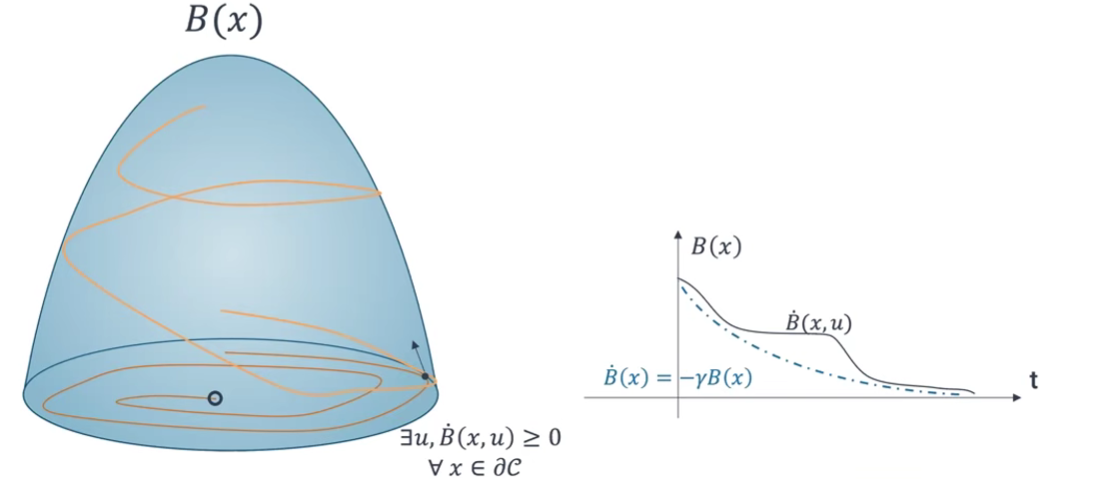
\includegraphics[width=\textwidth]{figures/cbf_geometry.png}
\caption[Barrier geometry and boundary behavior]{Barrier geometry and boundary behavior. The safe region satisfies $B(x)\geq0$. On its boundary, an admissible input must satisfy $\dot B(x,u)\geq0$; inside, a controlled decrease of $B$ is permitted.}
\label{fig:cbfgeometry}
\end{figure}

CBFs are a conceptual dual of the CLFs introduced in Section~\ref{ch:navigation}: a CLF decreases toward a target, whereas a CBF prevents departure from a set. A robot can remain safe without reaching its goal, or converge to a goal along an unsafe route. These objectives are therefore complementary.

For obstacle avoidance, the safe set can encode a required clearance around the robot rather than only the obstacle's visible surface. A configuration outside this region is inadmissible even if no contact has yet occurred. The chosen set should reflect the physical task and the information available to evaluate it.

Forward invariance connects a local condition on the current motion to the preservation of the set over time. The boundary matters because crossing it changes a safe state into an unsafe one. Inside the set, the robot retains freedom to move toward its task objective~\cite{litAmes2019}.

\subsection{The Barrier Condition}
For the nominal dynamics $\dot x=f(x)+g(x)u$, the chain rule gives
\begin{equation}
\dot B(x,u)=L_fB(x)+L_gB(x)u,
\quad L_fB=\nabla B^\top f,\quad L_gB=\nabla B^\top g.
\end{equation}
A continuously differentiable function $B$ is a CBF on a domain containing $\mathcal C$ if an admissible input can satisfy
\begin{equation}
L_fB(x)+L_gB(x)u\geq-\alpha(B(x)),
\label{eq:cbfcondition}
\end{equation}
where $\alpha$ is an extended class-$\mathcal K$ function: it is continuous, strictly increasing, and $\alpha(0)=0$~\cite{litAmes2017}. Unlike requiring $\dot B\geq0$ everywhere, this condition permits motion toward the boundary while limiting the approach rate.

For $\alpha(B)=\kappa B$, $\kappa>0$, direct integration yields
\begin{equation}
\frac{d}{dt}\left(e^{\kappa t}B(x(t))\right)\geq0
\quad\Longrightarrow\quad
B(x(t))\geq e^{-\kappa t}B(x(0))\geq0.
\end{equation}
The bound applies when the inequality holds along the trajectory and $B(x(0))\geq0$. More generally, forward invariance follows under the CBF theorem's regularity assumptions: locally Lipschitz dynamics and enforcing feedback, a regular boundary, and feasible inputs. The guarantee holds over the solution's existence interval; forward completeness extends it to all future time~\cite{litAmes2017}.

The function $\alpha$ determines how the allowed approach rate changes with the barrier value. Far from a constraint, the controller may have considerable freedom; closer to the boundary, the condition limits motion that would consume the remaining margin too quickly. This goes beyond checking whether the current position is collision-free.

Feasibility connects the geometry of the safe set to the available control authority. If the robot cannot brake strongly enough, a formally written inequality may demand an unavailable command. The existence of an admissible input is therefore part of the safety argument.

\subsection{Filtering a Learned Control Input}
Let $u_{\rm RL}$ be the command proposed by the navigation policy. A CBF filter selects a nearby admissible command by solving
\begin{equation}
\begin{aligned}
u^*(x)=\argmin_{u\in\mathcal U}\quad&\frac12\norm{u-u_{\rm RL}}^2\\
\text{subject to}\quad&L_fB(x)+L_gB(x)u\geq-\alpha(B(x)).
\end{aligned}
\label{eq:cbfqp}
\end{equation}
For a closed convex input set and a feasible constraint, this projection preserves an already admissible command and otherwise makes the smallest Euclidean correction. A CLF inequality can be included to encourage convergence, usually with a relaxation variable so that the stability objective can yield to the safety constraint~\cite{litAmes2017}.

The filter's guarantee depends on the model used in its constraint. For the disturbed dynamics of Section~\ref{ch:navigation}, the actual derivative contains the additional term $\nabla B(x)^\top d(t)$. Unknown wind must therefore be estimated or bounded when constructing the safety condition. Likewise, continuous-time enforcement does not follow from checking the inequality only at discrete control updates.

For several obstacles, the filter can include a condition for each relevant boundary. An action that is acceptable with respect to one obstacle may conflict with another, so the constraints must be considered together. An already admissible command is preserved, allowing the task policy to determine ordinary motion while the filter intervenes near active constraints.

The objective measures correction size; the constraints express safety. A nearby command is useful only if it satisfies those constraints.

\clearpage
\subsection{High-Order Control Barrier Functions}
A constraint has relative degree $r$ when the control input first appears in its $r$th time derivative. If $r>1$, the first-order condition cannot directly select $u$. High-order control barrier functions (HOCBFs) address this by recursively defining~\cite{litXiao2019}
\begin{equation}
\psi_0(x)=B(x),\qquad
\psi_i(x)=\dot\psi_{i-1}(x)+\alpha_i(\psi_{i-1}(x)),
\quad i=1,\ldots,r.
\end{equation}
Here the $\alpha_i$ are sufficiently smooth class-$\mathcal K$ functions. The final expression $\psi_r(x,u)$ contains the input. Enforcing $\psi_r\geq0$ preserves the intersection
\begin{equation}
\mathcal C_r=\bigcap_{i=0}^{r-1}\{x:\psi_i(x)\geq0\},
\end{equation}
provided the initial state lies in this intersection, the functions are sufficiently smooth, and a feasible regular feedback enforces the condition. Recursively applying the comparison argument then preserves each $\psi_i\geq0$, including $B\geq0$~\cite{litXiao2019}.

A braking example gives the intuition. Two vehicles can be at the same distance from a wall while having different opportunities to avoid it: one is nearly stationary, while the other approaches rapidly. A position-only snapshot treats their clearance equally, but a higher-order condition also accounts for how that clearance is changing. The controller must act early enough for the dynamics to respond.

\clearpage
For a simple acceleration-controlled navigation model, consider
\begin{equation}
\dot p=v,\qquad\dot v=u,\qquad
B(p)=\norm{p-p_o}^2-R^2,
\end{equation}
where $p_o$ is a fixed obstacle center and $R>0$ is the exclusion radius. Writing $e=p-p_o$ gives
\begin{equation}
\dot B=2e^\top v,\qquad
\ddot B=2\norm{v}^2+2e^\top u.
\end{equation}
The acceleration input appears only in the second derivative. With linear functions $\alpha_i(s)=k_i s$, $k_i>0$, the HOCBF constraint becomes
\begin{equation}
\ddot B+(k_1+k_2)\dot B+k_1k_2B\geq0.
\label{eq:hocbfsecondorder}
\end{equation}
Its initial conditions include both $B\geq0$ and $\dot B+k_1B\geq0$: clearance alone is insufficient when the robot approaches an obstacle too quickly. This explains the relevance to drones and other mechanical systems. The required relative degree depends on the chosen safety function and control interface, rather than the robot's name. Actuator limits can still make the HOCBF constraint infeasible.

\begin{figure}[H]
\centering
\begin{tikzpicture}[x=1cm,y=1cm,>=Stealth,font=\small]
\fill[gray!35] (9,-.45) rectangle (9.55,2.45);
\draw[gray!70,thick] (9,-.45)--(9,2.45);
\node[anchor=south] at (9.25,2.6) {Obstacle};
\draw[dashed,gray!65] (5,-.45)--(5,2.5);
\node[anchor=west] at (0,2) {Slow approach};
\node[anchor=west] at (0,0) {Fast approach};
\fill[teal] (5,2) circle (.13);
\fill[teal] (5,0) circle (.13);
\draw[->,very thick,teal] (5.2,2)--(6.15,2);
\draw[->,very thick,teal] (5.2,0)--(8.15,0);
\draw[<->,black!70] (5,-.85)--node[below]{Same clearance}(9,-.85);
\end{tikzpicture}
\caption[Clearance and approach speed]{Equal geometric clearance can require different braking responses. The arrows represent approach velocity: the faster state needs earlier intervention under limited acceleration.}
\label{fig:hocbfbraking}
\end{figure}

\FloatBarrier
\section{Reinforcement Learning with Control Barrier Functions}
\label{ch:rlcbf}

\subsection{Task Learning with a Safety Layer}
RL and CBFs give complementary responsibilities to an embodied controller. The RL policy chooses actions to accomplish a task, such as following a route or reaching a goal. The CBF layer checks those actions against a safety condition and corrects them when necessary. The policy supplies task-directed behavior; the filter restricts the commands applied to the robot.

For the nominal policy command $u_{\rm RL}$, this architecture is
\begin{equation}
u_{\rm RL}=\pi_\theta(o),\qquad
u_{\rm applied}=\operatorname{CBFfilter}(x,u_{\rm RL}),
\end{equation}
where $o$ is the policy observation and $x$ is the state information used by the filter. Under the assumptions of Section~\ref{ch:cbf}, continuous enforcement of a feasible CBF constraint guarantees forward invariance of the safe set. This provides a formal safety layer around learned decisions. The guarantee requires a valid model, safe initialization, and an implementation that enforces the condition; combining two modules alone is insufficient.

\begin{figure}[htbp]
\centering
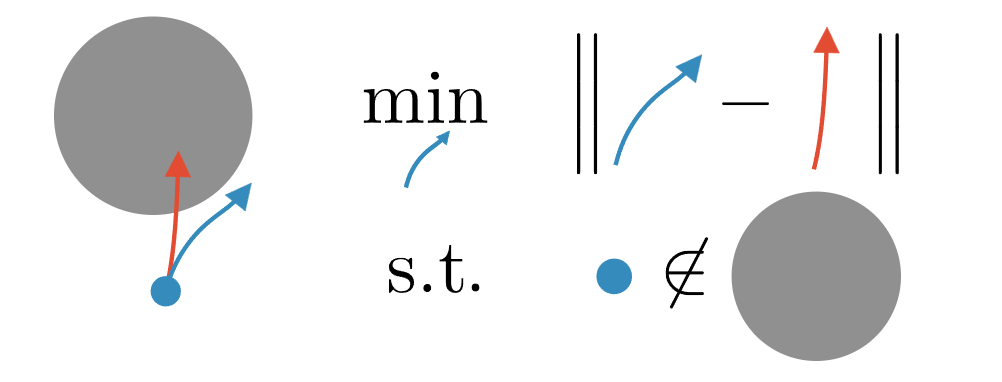
\includegraphics[width=.90\textwidth]{figures/pncbf_filter_concept.png}
\caption[Safety filtering of a nominal action]{Safety filtering of a nominal action. The red command points toward an obstacle; the blue correction preserves safety while remaining close to it. Illustration by So et al., PNCBF project page~\cite{litPNCBFProject}.}
\label{fig:rlcbfconcept}
\end{figure}

This division of responsibilities allows the policy to choose among several ways to accomplish a task while the filter excludes inadmissible commands. A correction is local to the current decision; it does not replace route planning or guarantee that every safe action eventually reaches the goal.

The components also need consistent information. The nominal command must use the same control coordinates as the filter output, and the barrier must be evaluated with an appropriate state estimate. Otherwise, the optimized correction may not correspond to the intended change in physical motion.

\subsection{Learning with CBF Corrections}
CBF-RL integrates the safety mechanism into training~\cite{litCBFRL2026}. Its \emph{Filter Only} variant corrects policy actions before execution. \emph{Reward Only} uses a barrier-inspired reward, while \emph{Dual} combines filtering and reward shaping. The reward encourages the policy to propose actions that need less correction. \emph{Nominal} provides the comparison without these additions.

Applying corrections during training changes the experience collected by the policy. A proposed action can produce a transition governed by the filtered action. CBF-RL combines this intervention with reward shaping so that the policy can learn to propose commands requiring fewer corrections~\cite{litCBFRL2026}.

\begin{figure}[htbp]
\centering
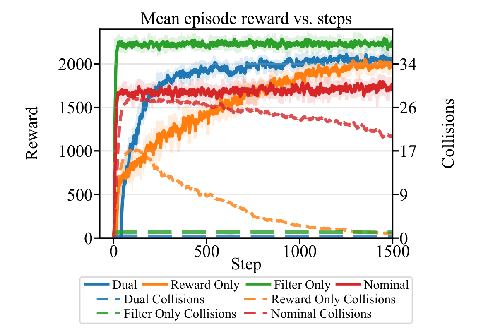
\includegraphics[width=.66\textwidth]{figures/cbfrl_training_original.pdf}
\caption[Training reward and collisions in CBF-RL]{Training reward and collisions in the 2D navigation experiment of Yang et al.~\cite{litCBFRL2026}, Fig.~3. Solid curves show rewards and dashed curves show collisions. These are the authors' experimental results.}
\label{fig:rlcbftraining}
\end{figure}

Figure~\ref{fig:rlcbftraining} shows rapid reward improvement and substantially fewer training collisions with filtering. Filter Only reaches a high reward early, while Dual improves faster than Reward Only over much of training. The horizontal axis measures training steps, not elapsed computation time.

The paper also evaluates deployment without a filter: Filter Only degrades markedly when its filter is removed. Empirical policy safety therefore does not replace the guarantee of an actively enforced CBF~\cite{litCBFRL2026}.

The comparison separates safer exploration from improvements in the policy itself. Fewer training collisions can make data collection more useful, but it remains necessary to identify which mechanism is active during execution. Evaluating a policy with and without its runtime filter reveals how much of the observed behavior depends on that intervention.

\subsection{Barrier Learning with Policy Neural CBFs}
A complementary approach learns the safety function itself. Policy neural CBFs (PNCBFs) approximate a nominal policy's maximum-over-time safety cost from rollouts, then use this value function to support safety filtering~\cite{litPNCBF2023}.

So et al. demonstrate the approach on a 16-dimensional F-16 model and two quadrotors in hardware~\cite{litPNCBF2023}. These examples illustrate the reach of learned safety filters, although approximation accuracy and CBF validity remain necessary for a formal guarantee.

The maximum-over-time cost accounts for unsafe behavior that may occur later in a trajectory. A policy can initially move away from an obstacle and still encounter another constraint farther along its route. Rollouts therefore provide information beyond current geometric clearance.

Learning a barrier is attractive when constructing one by hand is difficult. However, learning a useful representation and verifying its barrier property remain distinct tasks. The neural model approximates the relevant function; the safety argument depends on the conditions satisfied by that approximation~\cite{litPNCBF2023}.

\subsection{Disturbance Randomization and Wind Robustness}
The 2D navigation experiment in CBF-RL randomizes dynamics using additive Gaussian perturbations~\cite{litCBFRL2026}. This does not establish robustness to persistent wind or gusts. Turbulence models introduce temporal structure: Dryden filters shape white noise into correlated gust signals~\cite{litDryden2018}. Gaussianity alone therefore does not describe a disturbance's temporal behavior.

The disturbance time scale matters because feedback needs time to respond. Independent perturbations can partly cancel across successive steps, while a sustained force can displace the vehicle in one direction for longer. Testing across these structures helps distinguish tolerance to isolated deviations from adaptation to a changed operating condition.

For example, two disturbance sequences can have similar distributions of instantaneous values while differing in their ordering. One may change direction frequently, whereas the other may retain a directional bias over several control updates. The resulting motion need not be the same because the vehicle carries velocity and the controller reacts with finite delay. This illustrates why a histogram of disturbance magnitudes is not a complete description of a navigation test.

A useful evaluation therefore considers disturbance strength together with persistence, changes during a mission, and the available obstacle clearance. These choices help identify whether the controller merely tolerates sampled perturbations or responds effectively when conditions shift. The prior work in Section~\ref{ch:disturbanceprior} offers several ways to address that response.

This raises the question: \emph{can such a policy maintain reliable navigation and safety under persistent wind, gusts, and disturbance shifts beyond training conditions?}

\FloatBarrier
\section{Navigation Under Disturbance}
\label{ch:disturbanceprior}

Wind can displace a robot from its planned trajectory even when the nominal navigation policy performs well. Rejecting that disturbance requires the controller to respond to effects that may be uncertain, persistent, or changing during flight. Classical approaches use feedback, estimation, and robust design; learning methods add representations or policies that can adapt from experience. The following works mainly address motion control and trajectory tracking, which support navigation but do not by themselves guarantee obstacle avoidance.

\subsection{Classical Methods}

\FloatBarrier
\subsubsection{\texorpdfstring{$\mathcal L_1$}{L1} Adaptive Control}
The $\mathcal L_1$ architecture of Cao and Hovakimyan combines rapid adaptation with a low-pass filter in the control channel~\cite{litL1Original2006}. A state predictor measures the discrepancy between expected and observed motion. An adaptation law estimates the uncertainty, while the filter limits the frequency content of the resulting control correction. This separates fast estimation from the bandwidth of the commands sent to the actuators.

The original analysis establishes transient tracking bounds for its uncertain linear-system setting under a small-gain condition and bounded-parameter assumptions. In quadrotor control, Hanover et al. combine an $\mathcal L_1$ augmentation with nonlinear MPC to compensate for model mismatch and payload changes~\cite{litHanover2022}. The practical design must balance disturbance rejection against sensor noise, delay, and actuator bandwidth.

The estimate need not identify the physical origin of every mismatch. For navigation, its immediate purpose is to support a suitable correction. This makes the architecture useful when payload changes or external forces alter the response, provided those effects remain compatible with the assumptions of the chosen augmentation.

\FloatBarrier
\subsubsection{Incremental Nonlinear Dynamic Inversion (INDI)}
INDI uses measured acceleration to determine how much the control input should change. Instead of reconstructing every aerodynamic force, it starts from the vehicle's observed response and uses a local control-effectiveness model to compute an input increment. Disturbances are therefore reflected in the measured motion and compensated through feedback.

Smeur et al. develop adaptive INDI for micro-air-vehicle attitude control, then extend it to a cascaded structure for disturbance rejection~\cite{litINDI2016,litINDI2018}. The outer loop turns a desired translational acceleration into thrust and attitude commands; the inner loop controls attitude. This reduces dependence on a detailed aerodynamic model, although it still requires reliable acceleration measurements, control-effectiveness estimates, and careful alignment of filtering and actuator dynamics.

Measurement timing is particularly important in an incremental method. Comparing a recently measured acceleration with an input associated with an earlier actuator response can produce a misleading correction. Synchronizing the relevant signals helps the controller interpret the observed motion consistently~\cite{litINDI2016}.

\FloatBarrier
\subsubsection{Disturbance Observers (DOB) and Exponential Smoothing}
A disturbance observer estimates the difference between a nominal model's predicted response and the measured response. Ohnishi's early servo architecture uses estimated load torque to compensate its effect on motion~\cite{litDOB1987}. More generally, the estimate combines external disturbances and model mismatch into an equivalent disturbance, avoiding separate identification of every aerodynamic contribution.

Filtering is central to this design. Sariyildiz and Ohnishi show that measurement filtering affects the stability and robustness of a DOB and constrains its usable bandwidth~\cite{litDOB2015}. A higher observer bandwidth can track faster disturbances, but also exposes the controller to measurement noise and neglected dynamics.

An exponential moving average (EMA) is a simple first-order smoothing option for a sampled disturbance estimate: each update blends the new estimate with its previous filtered value. Stronger smoothing suppresses rapid fluctuations but delays the response to gusts. EMA is a filtering component, not a complete observer; the model and measurements must first supply an estimate to filter. Its suitability depends on the disturbance time scale and the available feedback rate.

A filtered estimate can therefore remain smooth while temporarily lagging a changing disturbance. Its usefulness should be assessed together with the resulting motion, rather than from smoothness alone. This links observer design to the clearance and recovery time available in the navigation task.

\FloatBarrier
\subsubsection{\texorpdfstring{$H_\infty$}{H-infinity} Robust Control}
$H_\infty$ control approaches disturbance rejection through a worst-case performance criterion. In the formulation of Doyle et al., the external input $w$ includes disturbances and measurement noise, while the regulated output $z$ represents weighted errors and other performance objectives~\cite{litHinf1989}. The controller limits the closed-loop amplification from $w$ to $z$, measured by its induced energy gain. It therefore does not require a specific Gaussian disturbance distribution.

The seminal state-space result constructs controllers for a finite-dimensional linear time-invariant model using algebraic Riccati equations. For flight control, the designer must choose a suitable model and performance weights, balancing tracking accuracy, disturbance attenuation, and control effort. The resulting bound concerns the modeled input-output behavior; it does not establish collision avoidance for an arbitrary nonlinear vehicle under unlimited wind.

The performance weights determine which errors the design prioritizes. For example, reducing position error more aggressively can require greater control effort. Robust synthesis makes that trade-off explicit within the model; the selected weights and available actuators determine whether the resulting design is useful for a particular vehicle.

\subsection{Learning Methods}
Deep learning makes it possible to represent complex dynamics and train controllers across varied operating conditions. The methods below differ in what adapts: an adversarially trained policy, a latent description of the environment, an aerodynamic force model, or the policy parameters.

\FloatBarrier
\subsubsection{Adversarial Reinforcement Learning: REFORMA}
REFORMA trains a drone controller against a group of adversaries that perturb its actions~\cite{litREFORMA2024}. The protagonist learns to complete hovering and traversal tasks while the adversaries seek to reduce its return. Training emphasizes the average performance against the adversaries inducing the lowest protagonist returns, exposing the controller to challenging interactions beyond randomly sampled perturbations.

The adversary strength $\alpha$ controls the mixing of protagonist and adversary actions. A factor encoder forms $z_t$ from environment parameters, states, and protagonist and attacked actions. An adaptation module predicts this representation from recent state/action histories to condition the policy at deployment. Neither module receives $\alpha$ explicitly; disturbance strength is inferred through the observed interaction (Figure~\ref{fig:reforma}).

\begin{figure}[H]
\centering
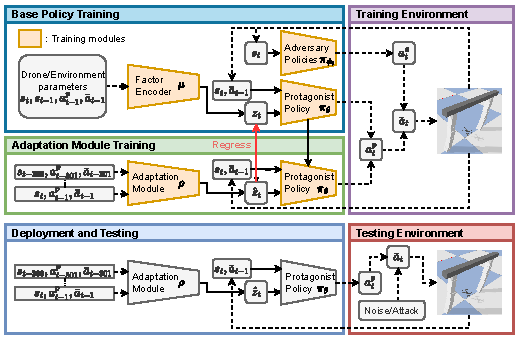
\includegraphics[width=.96\textwidth]{figures/reforma_architecture.pdf}
\caption[REFORMA training and adaptation]{REFORMA: adversarial policy training, adaptation-module training, and deployment. From Hsu et al.~\cite{litREFORMA2024}, Fig.~1. Symbols retain the authors' notation.}
\label{fig:reforma}
\end{figure}

The authors evaluate the method in simulation. Their results support robustness to the tested action disturbances, but the adversary's action space and strength still define which challenges training can represent. Adversarial training does not automatically cover every physical wind field.

Using several adversaries broadens the challenging interactions encountered during training. However, they still act through the disturbance mechanism defined by the environment. This makes the design of the adversary meaningful: robustness to an action perturbation should be interpreted in relation to the physical effect that perturbation is intended to represent.

\FloatBarrier
\subsubsection{Rapid Motor Adaptation (RMA)}
Rapid Motor Adaptation separates a base policy from a module that infers the current operating conditions~\cite{litRMA2021}. Kumar et al. introduce this architecture for quadruped locomotion at RSS 2021. Its relevance to flight is the general adaptation principle: recent motion contains information about dynamics that are not directly measured.

\begin{figure}[H]
\centering
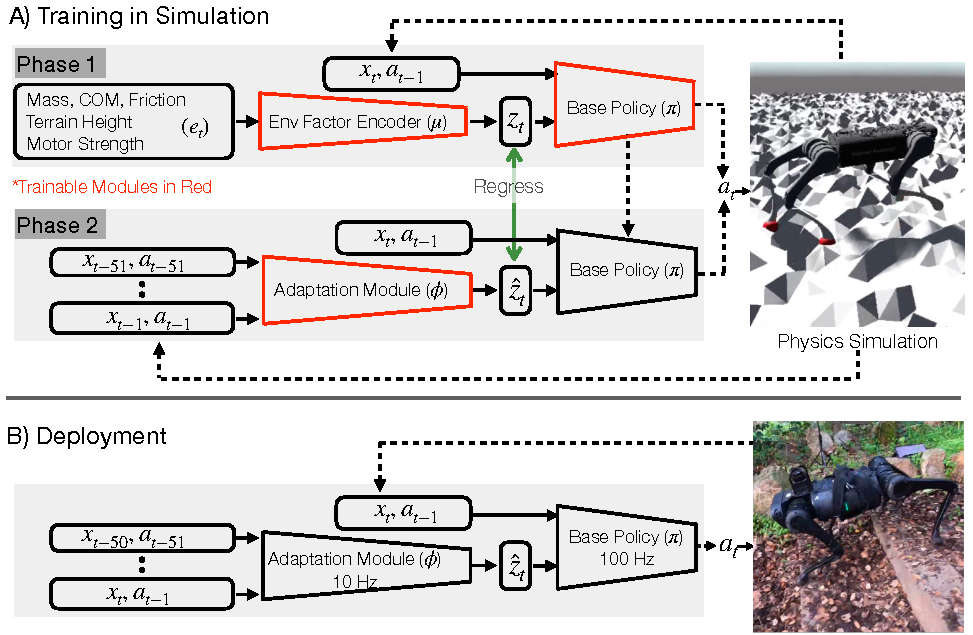
\includegraphics[width=\textwidth]{figures/rma_architecture.pdf}
\caption[Rapid Motor Adaptation architecture]{RMA's two training phases and deployment architecture. From Kumar et al.~\cite{litRMA2021}, Fig.~2. The adaptation module estimates the latent operating conditions used by the base policy.}
\label{fig:rma}
\end{figure}

\Needspace{3\baselineskip}
During simulation training, an encoder $\mu$ converts privileged environmental factors $e_t$, such as friction and payload, into a latent vector $z_t$. The policy $\pi$ uses this vector alongside the robot state and previous action. A second training phase teaches an adaptation module $\phi$ to estimate $\hat z_t$ from a history of states and actions. Deployment uses this estimate instead of privileged simulator information.



RMA adapts its latent input online without retraining the policy weights on the robot. The authors demonstrate locomotion over varied real terrain and changing conditions. These experiments establish a useful precedent for adaptation from motion history, while their legged-robot results are not a direct evaluation of aerial wind rejection.

The latent vector need not recover each physical parameter separately. It needs to retain information that helps the policy select an appropriate response. This reduces the burden of explicit identification, although ambiguous or unfamiliar motion histories can still make adaptation difficult~\cite{litRMA2021}.

\FloatBarrier
\subsubsection{Neural-Fly: Learned Aerodynamics with Adaptive Control}
Neural-Fly combines a learned aerodynamic representation with a structured online adaptation law~\cite{litNeuralFly2022}. O'Connell et al. train a neural basis using flight data from different wind conditions. Their domain-adversarially invariant meta-learning procedure seeks a shared representation whose coefficients can change with the wind.

Using the authors' notation, the force estimate has the form $\hat f=\phi\hat a$: the learned basis $\phi$ is fixed during deployment, while the coefficients $\hat a$ adapt online. The update uses both tracking error and force-prediction error. This retains a conventional feedback controller and concentrates online learning in a compact set of parameters.

\begin{figure}[H]
\centering
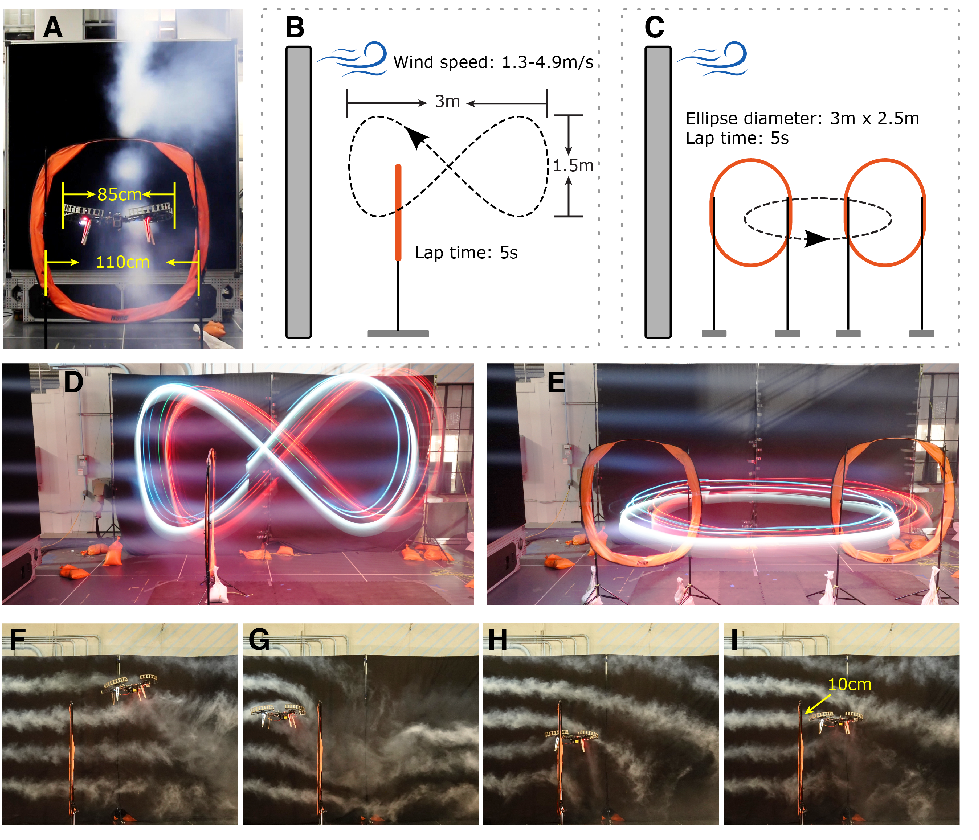
\includegraphics[width=.86\textwidth]{figures/neuralfly_flight.pdf}
\caption[Neural-Fly flight experiments]{Wind-tunnel setup, reference trajectories, and gate-passing photographs from O'Connell et al.~\cite{litNeuralFly2022}, Fig.~1. These panels illustrate the authors' physical flight experiments.}
\label{fig:neuralfly}
\end{figure}

The Science Robotics study reports experiments in winds up to $12.1\,\mathrm{m\,s^{-1}}$ and improved tracking over its comparison controllers. Its gate experiments illustrate precise flight under wind, while its stability analysis bounds the effect of imperfect learning under stated assumptions. Neural-Fly is a learning-based adaptive controller; its domain-adversarial representation learning is distinct from REFORMA's adversarial RL action perturbations.

The compact online update is a central design choice. The learned basis captures reusable aerodynamic structure, while the changing coefficients respond to the current conditions. This gives the adaptive part a clear role inside the feedback loop without retraining the entire representation during each flight~\cite{litNeuralFly2022}.

\FloatBarrier
\subsubsection{DATT: Deep Adaptive Trajectory Tracking}
DATT combines feedforward trajectory information, state feedback, and disturbance adaptation in an RL policy~\cite{litDATT2023}. A learned encoder summarizes upcoming reference positions, allowing the policy to anticipate turns. State feedback describes the current motion, while a disturbance input tells the controller how the observed dynamics differ from the nominal model.

\begin{figure}[H]
\centering
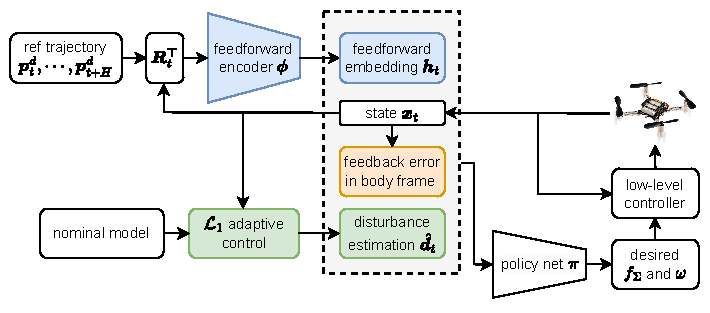
\includegraphics[width=\textwidth]{figures/datt_architecture.pdf}
\caption[DATT feedforward, feedback, and adaptation]{DATT architecture from Huang et al.~\cite{litDATT2023}, Fig.~2. Blue, yellow, and green identify feedforward, feedback, and adaptation components. The authors distinguish the simulated disturbance $d$ from its runtime estimate $\hat d$.}
\label{fig:datt}
\end{figure}

The policy is trained with PPO in simulation and deployed with an $\mathcal L_1$ disturbance estimator, without policy fine-tuning on hardware. It outputs collective thrust and desired body rates. Experiments include smooth references, sharp-turning trajectories that cannot be followed exactly, and unsteady wind. The objective is to reduce tracking error within the vehicle's capabilities, not to make an infeasible reference physically feasible.

DATT already introduces temporal structure into training disturbances: its disturbance follows a Brownian random walk with Gaussian increments. This is an important distinction from independent additive samples. Consequently, temporally correlated disturbance training is established prior work. The remaining question concerns how well adaptation and safety mechanisms handle disturbance conditions beyond those represented during training.

Looking ahead along the reference helps the controller prepare for a turn before the tracking error becomes large. The disturbance estimate supplies different information: how current motion departs from the nominal response. DATT brings these anticipatory and reactive signals together in the same policy.

\FloatBarrier
\subsubsection{Learning on the Fly: Residual Models and Policy Adaptation}
Learning on the Fly (LoTF) updates a deployed policy through a differentiable simulator~\cite{litLoTF2026}. Pan et al. start with an analytical dynamics model and learn a residual model from recent flight data. Together they form a hybrid simulator that better matches the current vehicle and environment. Gradients through simulated rollouts then update the task policy.



The paper compares full policy adaptation with low-rank adaptation (LoRA). Full adaptation updates all policy parameters. LoRA freezes the pretrained parameters and learns an additive low-rank module, reducing the number of trainable parameters. Here, residual learning corrects the dynamics model; it should not be confused with simply adding a residual action to the controller output.

The authors demonstrate adaptation in simulation and physical flight under disturbances and model mismatch. Unlike RMA, LoTF changes policy parameters during deployment; unlike Neural-Fly, adaptation extends beyond force-estimation coefficients. Its performance depends on the quality of the updated simulator and the policy updates it produces.

\begin{figure}[H]
\centering
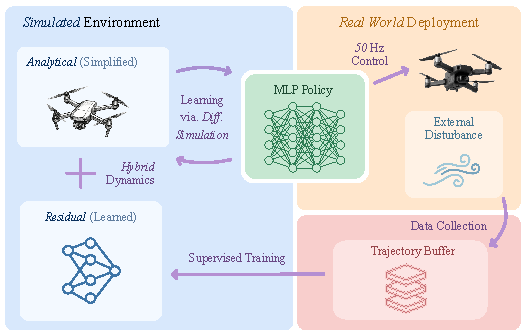
\includegraphics[width=.96\textwidth]{figures/lotf_architecture.pdf}
\caption[Learning on the Fly adaptation loop]{LoTF combines flight-data collection, residual dynamics learning, and policy adaptation through differentiable simulation. From Pan et al.~\cite{litLoTF2026}, Fig.~1. The diagram shows the authors' method.}
\label{fig:lotf}
\end{figure}

The rolling flight-data buffer creates a practical adaptation trade-off. Recent samples describe current conditions, while a broader history can stabilize model fitting. The learned model must remain useful for policy optimization as new data arrive; merely fitting the recent measurements is not the whole control objective.

These methods demonstrate several routes to adaptation, with different requirements for models, representative data and online updates. For a connected robot, a complementary objective is to make recent motion directly useful to a compact safety layer. Chapter~\ref{ch:contribution} develops this idea through disturbance estimation and residual uncertainty, using a rolling window of prediction errors to update the CBF safety margin.
